\chapter{GUI Windows}

%-----------------------------------------------------------------
\section{Parameter Input}
\label{s:param.input}

In general, real parameter values can be set using expressions just like parameter values can be set
using expressions on the \tao command line.

%-----------------------------------------------------------------
\section{The Main GUI Window}
\label{s:gui.root.window}

\begin{figure}
\centering
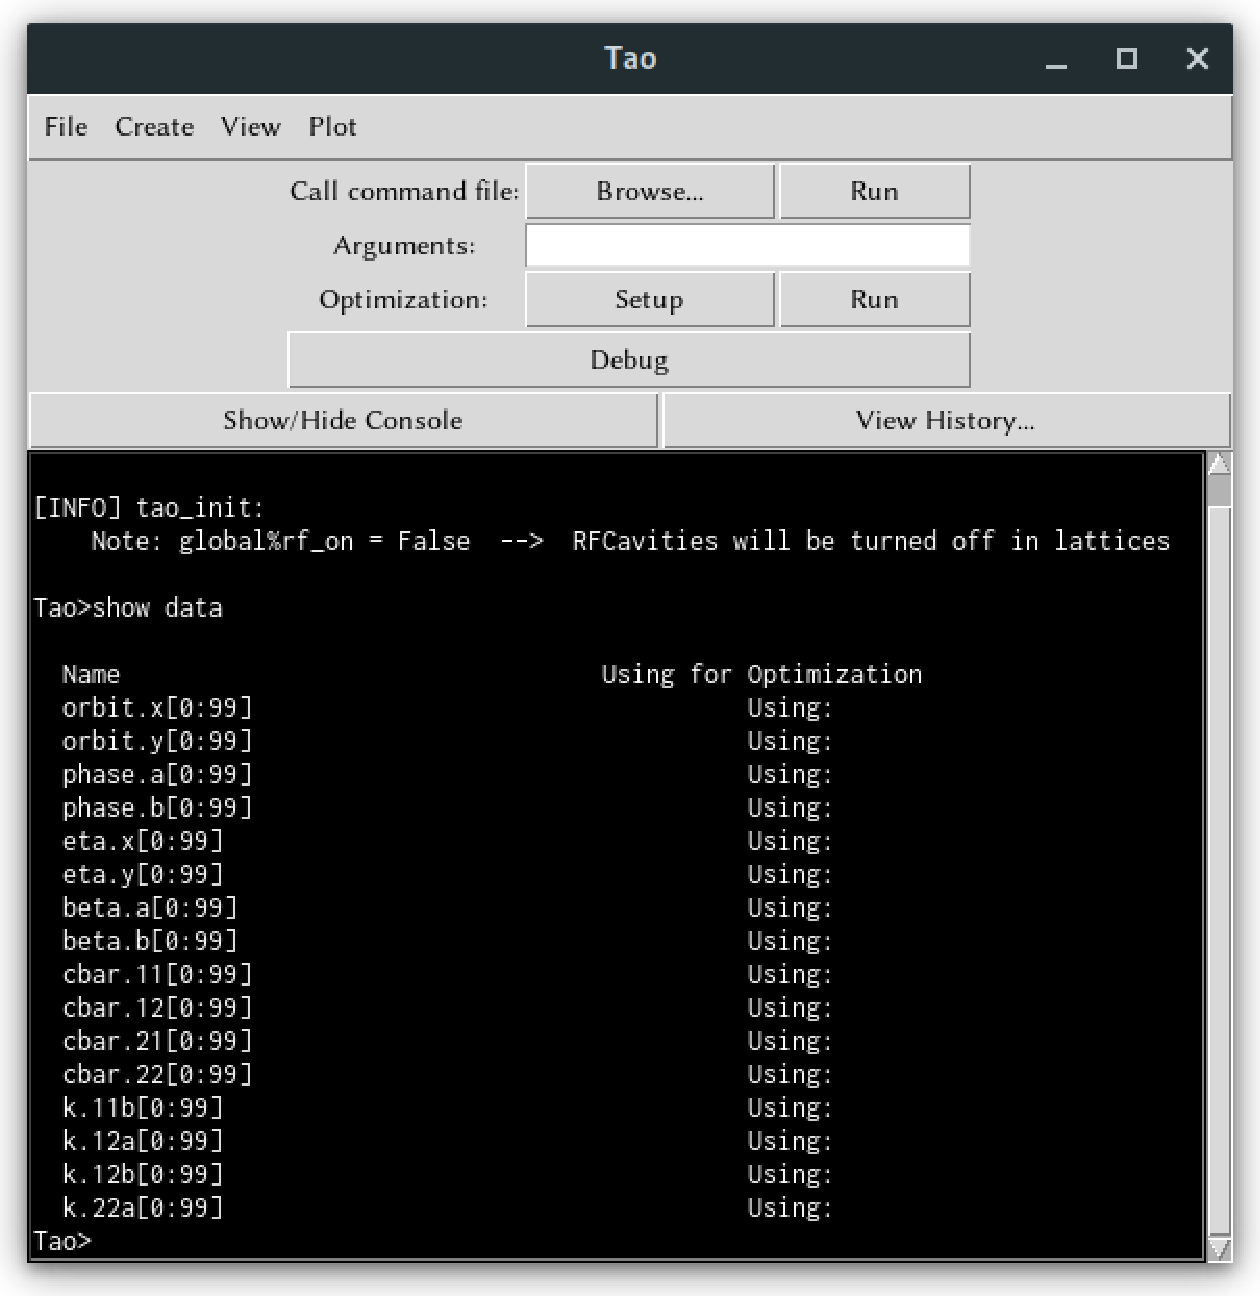
\includegraphics[width=8cm]{figures/root_window.pdf}
\caption[The main GUI window.]{The main GUI window, showing the results of \texttt{show data} on the console.}
\label{fig:root.window}
\end{figure}

The main window for the GUI is shown in Figure \ref{fig:root.window}.
From here, the user has access to all of the GUI's features.
Command files can be called by browsing for them and then clicking "Run", with arguments specified in the "Arguments" below.
In the future, the user will also be able to set up and run optimization routines from this window, although this feature is not currently available.

The main window also has a console, where commands can be run in Tao exactly like in regular Tao.
The console will also display warning messages if a command produces an error.

%-----------------------------------------------------------------
\section{Global Variables}
\label{s:gui.global.variables}

Global variables in Tao can be viewed and modified from the global variables window as shown in Figure \ref{fig:gui.global.variables}.
Once you have editted the global variables, clicking the "Set Global Variables" button will set the variables in Tao as appropriate.

\begin{figure}
\centering
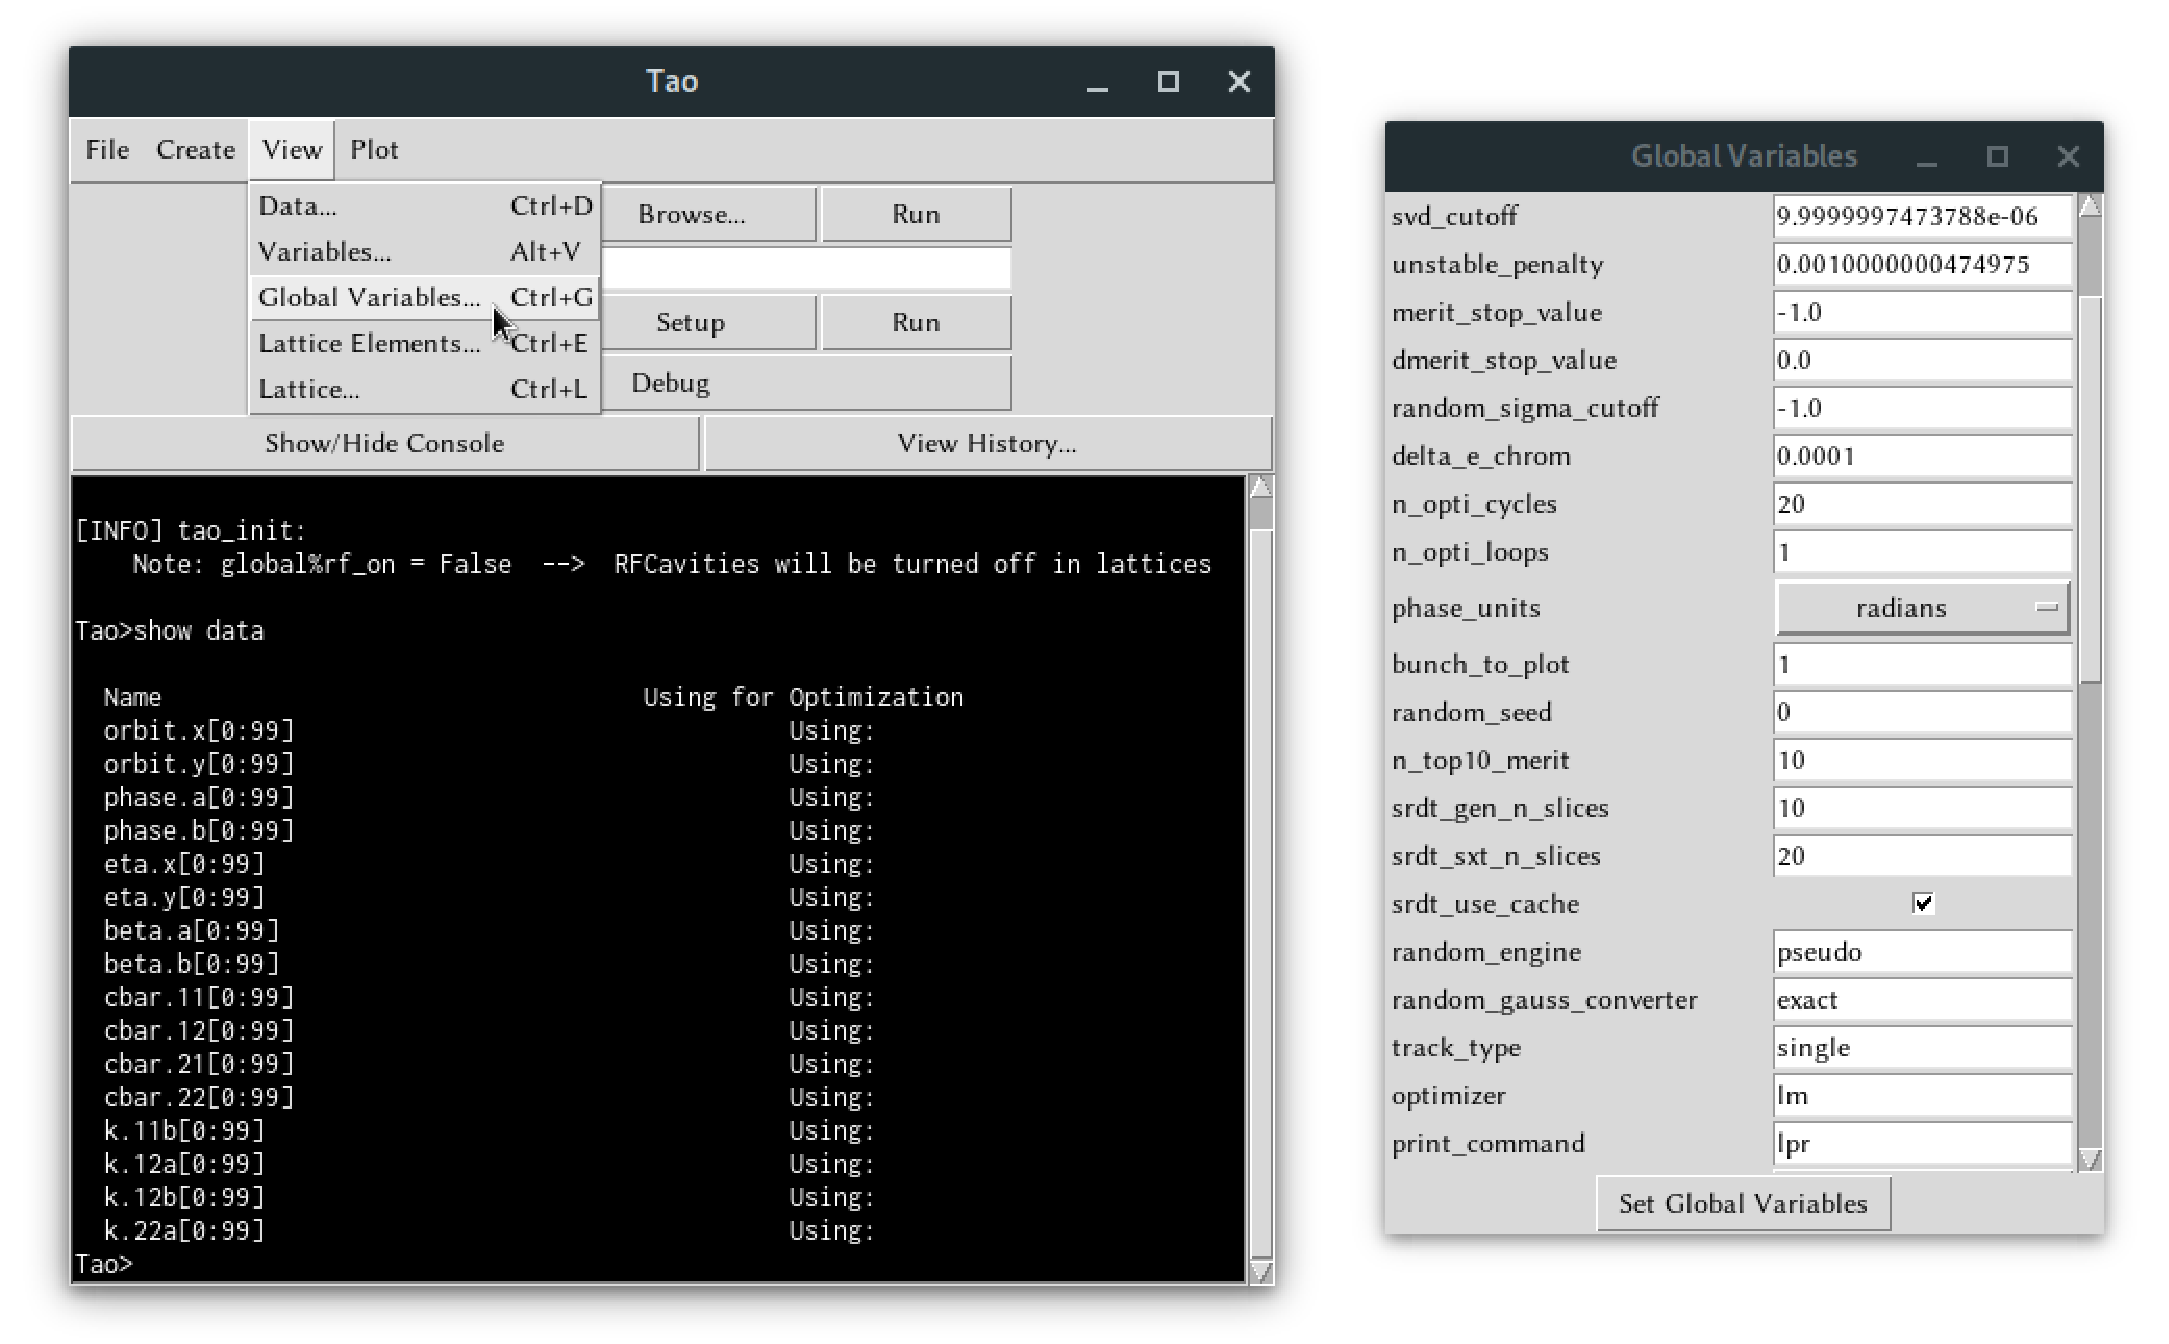
\includegraphics[width=10cm]{figures/globals.pdf}
\caption{View and edit global variables with the Global Parameters window.}
\label{fig:gui.global.variables}
\end{figure}

